When reconstructing GW signals to measure source parameters, we typically rely on a \textit{modelled} approach i.e. relying on GW signal models obtained by solving the field equations. However, there are cases where theoretical models either do not exist or are expensive to simulate. For such scenarios, it becomes important to be able to perform \textit{unmodelled} reconstruction. Here, we review how unmodelled reconstruction is done, particularly for a case where robust theoretical models do not exist. 

\section{Artefacts in Gaussian noise}
\label{sec:artefact}
\begin{figure}[h]
    \centering
    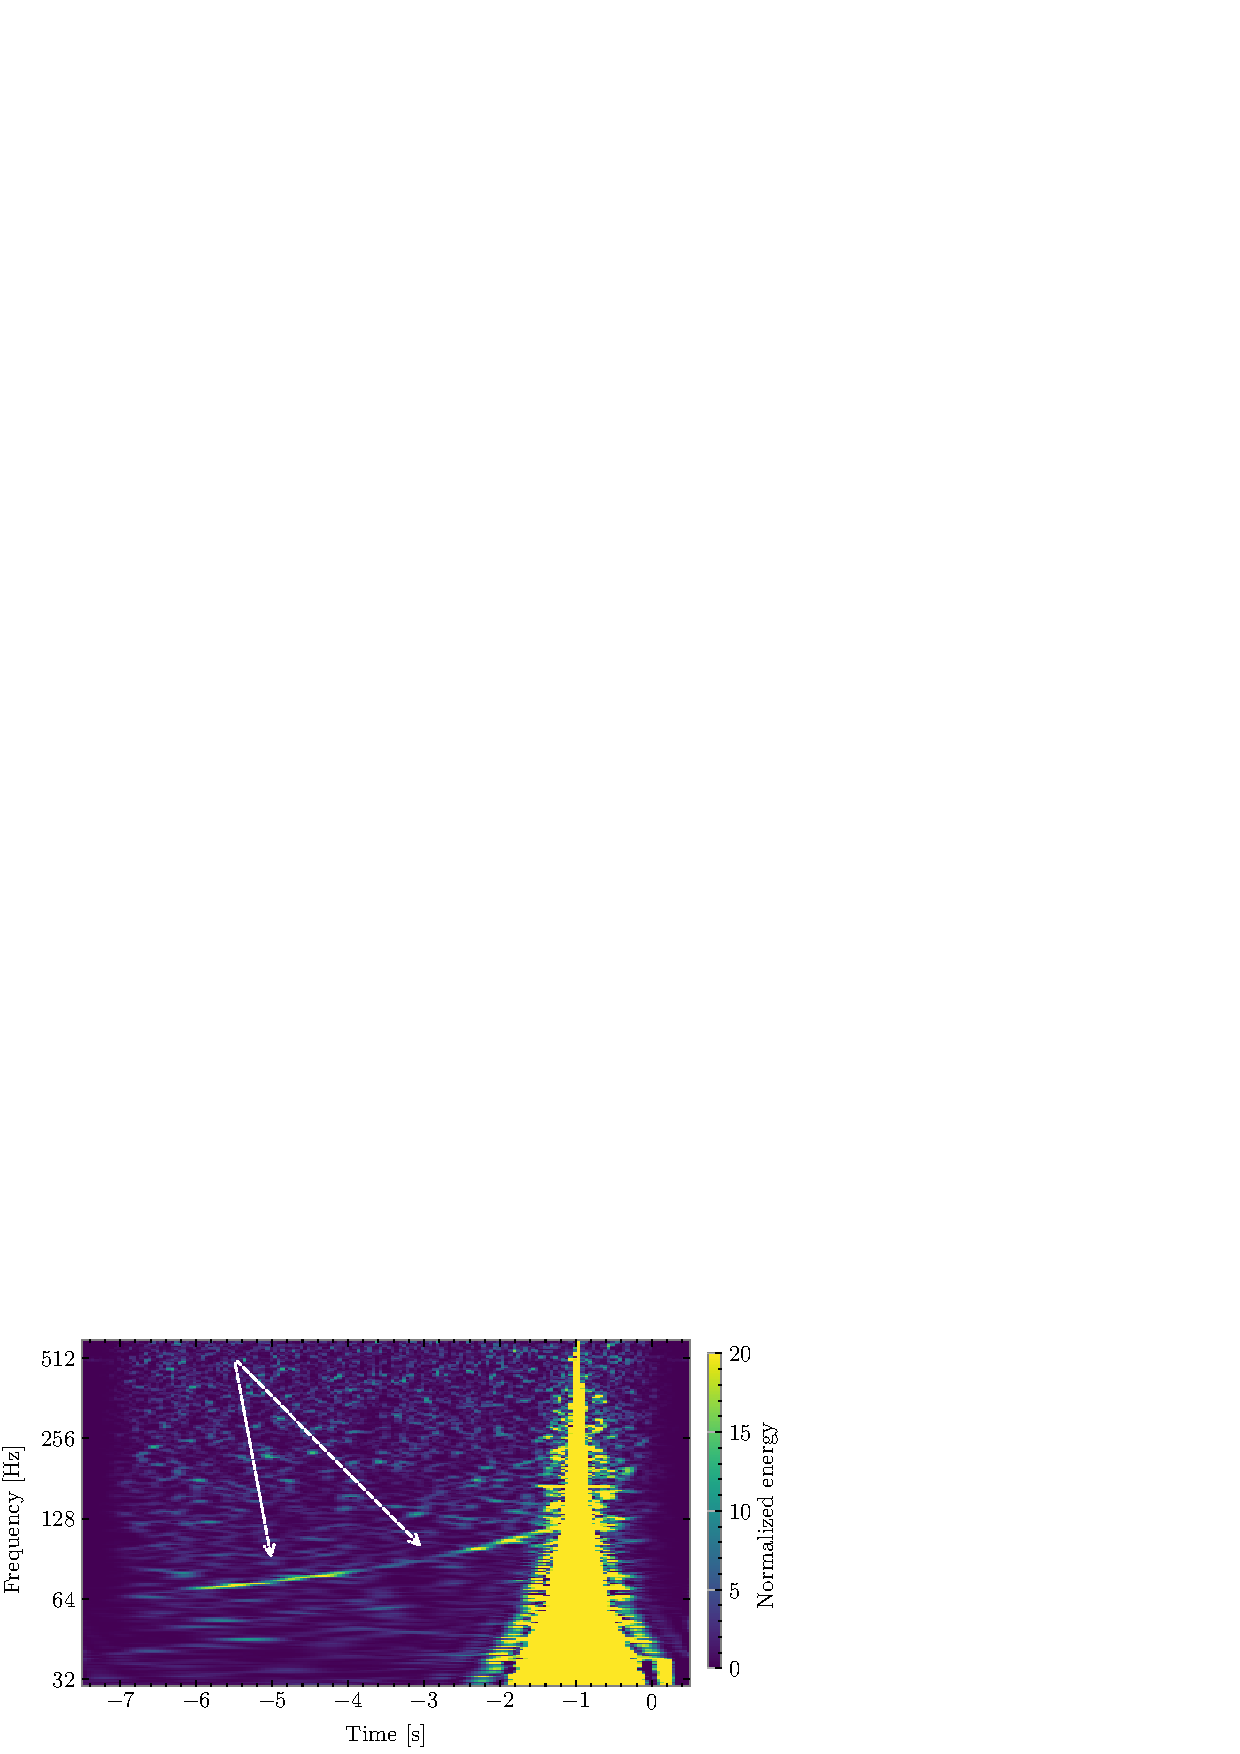
\includegraphics[width=12cm]{../figures/gw170817scan.png}
    \caption{A loud glitch overlapping with the binary neutron star signal, GW170817, in LIGO-Livingston interferometer. Dashed white arrows are added to help reader trace the signal.}
    \label{fig:bns_scan}
\end{figure}
A case where theoretical models do not exist can be made for instrumental noise transients or \textit{glitches}. While the background noise in the GW detectors is assumed to be Gaussian and stationary, occurrence of a glitch violates this assumption. As most of our physics inferences hinges on the assumption that background noise is Gaussian-stationry, a violation of it could corrupt the inferences. Depending on the time of occurrence, glitches can be problematic in two ways,
\begin{itemize}

\item \textit{Glitches overlapping with a GW signal.} Glitches occurring near a GW signal could corrupt the measurements of its source parameters. Therefore, it becomes necessary to carefully subtract the glitch without the contaminating the signal, \textit{before} we measure the source parameters. The first detection of a GW signal from merger of two neutron star (GW170817) is an example of this kind (Figure~\ref{fig:bns_scan}).
\begin{figure}
    \centering
    \includegraphics[width=12cm]{../figures/thesis-plot_highmass_blip_qscan.png}
    \caption{\textit{Left:} A GW signal emitted by a BBH merger with total mass of $176 M_{\odot}$. \textit{Right:} An isolated blip glitch.}
    \label{fig:bbh_blip}
\end{figure} 
\item \textit{Glitches in isolation.} Glitches not overlapping with a GW signal increase the false alarm rate of GW detections since some glitches look similar to a signal. For example, Figure~\ref{fig:bbh_blip} shows the time-frequency evolution of a GW signal from high-mass BBH mergers (left) and the time-frequency evolution of an isolated blip glitch (right). It becomes important to identify and veto glitchy data from the analysis to reduce false alarms.
\end{itemize} 


Glitches could be caused by instrumental (control systems, scattered light) or environmental (earthquakes, wind, anthropogenic) factors, though their origins often remain unknown in many cases. Therefore, it is not possible to devise a theoretical model for glitches in most cases. We need to rely on the unmodelled approach to reconstruct and subtract glitches. 

\iffalse
A case where theoretical model is expensive to simulate can be made for GW signals from the core collapse of a supernova. A case where theoretical models are not mature enough can be made for the echoes of GW signal. Why do we still do on-source PSD estimation? 
\fi

\section{Transdimensional Sampling Algorithms}
When performing unmodelled reconstruction, the dimensionality of the parameter space of $\vec{\theta}$ is unknown, in contrast to the modelled reconstruction explained in chapter~\ref{ch:gwpe}. While the Bayesian framework, GW likelihood, and Bayesian approximation still remain robust, the Nested sampling algorithm from previous chapter is not a suitable for the problem at hand. Here, we review a transdimensional algorithm that is routienly used to explore a variable dimensional parameter space. Let us define a few standard quantities which formulate building blocks of the algorithm. 
\subsection{Morlet-Gabor wavelets}
\begin{figure}
    \centering
    \includegraphics[width=12cm]{../figures/morlet_gabour.pdf}
    \caption{Morlet-Gabour wavelet in time (left) and frequency (right) domain}
    \label{fig:mg_wav}
\end{figure}
When performing unmodelled reconstruction, we use Morlet-Gabor wavelets as bases functions. It can be expressed in time domain as
\begin{equation}
    \label{eq:wavelet}
    \vec{\psi}(t; A, Q, t_0, f_0, \phi_0) = A~e^{-\frac{(t-t_0)^2}{2\tau^2}}~\sin{\left(2{\pi}f_0(t-t_0) + \phi_0\right)},
\end{equation}
where $t$ denotes time, $A$ denotes amplitude, $\tau = Q/(2{\pi}f_0)$ denotes the quality factor that controls the spread of the wavelet, $\phi_0$ denotes initial phase, $t_0$ and $f_0$ respectively correspond to time and frequency at the peak of the amplitude. In Figure~\ref{fig:mg_wav}, we show a time (left) and frequency (right) domain representation of a wavelet with parameters $Q = 20$, $t_0=1$ second, and $f_0 = 40$ Hz. 

Morlet-Gabor wavelets are sutible for the problem at hand because glitches $(\vec{g})$ we want to reconstruct can be expressed as linear combination of $N$ wavelets [BayesWave first paper],
\begin{equation}
    \vec{g}(t; \vec{\theta}) = \sum_{k = 0}^{N} \vec{\psi}_k(t; \vec{\theta}_k),
\end{equation}
where $\vec{\theta}$ is set of $N\times5$ parameters since each $\vec{\psi}_k$ needs 5 model parameters shown in Eq.~\eqref{eq:wavelet}. A desirable feature is that Morlet-Gabor wavelets preserve shape when switching between time-frequency domains and they have a simple analytic expression in both domains.

Besides ${\vec{\theta}}$, here $N$ itself is an unknown parameter therefore the dimensionality of the parameter space we want to explore is also unknown. The transdimensional algorithm used to tackle this problem is an extension of the Markov chain Monte Carlo methods. 

\subsection{Markov chain Monte Carlo}
Markov chain Monte Carlo (MCMC) is a subclass of Monte Carlo methods, a class of computational methods that rely on repeated random sampling. Markov chain in particular refers to an iterative process where the probability  of accepting a proposal at $t^{\mathrm{th}}$ iteration depends only on the point from previous iteration. If we denote the probability by $p_t$, 

\begin{equation}
p_t(\vec{\theta}') = \int \mathrm{d}\vec{\theta}_{t-1}~T(\vec{\theta}', \vec{\theta}_{t-1})~\vec{\theta}_{t-1}
\end{equation}
where $\vec{\theta}'$ is the proposed point, $\vec{\theta}_{t-1}$ is the point from previous iteration, and $T$ is the transition probability. 

Traditional MCMC algorithms aim to obtain the samples from posterior probability distribution which is in contrast to the Nested sampling algorithm where the aim is to compute the evidence and posterior distributions are the byproduct. Obtaining the evidence after an MCMC algorithm is terminated requires additional computations. Nevertheless, here we outline one such MCMC algorithm called the Metropolis–Hastings algorithm.

\begin{figure}
    \centering
    \includegraphics[width=8cm]{../figures/markov_chain.pdf}
    \caption{\textit{Bottom:} Progression of a Markov chain in the parameter space of $\vec{\theta}$. Each arrow represents an iteration, solid black dots represent accepted proposal and empty dots represents rejected proposals. \textit{Top:} Posterior probability distribution constructed from the accepted samples of the Markov chain of the bottom plot.}
    \label{fig:mcmc}
\end{figure}
\subsubsection{Metropolis-Hastings algorithm}
Metropolis-Hastings algorithm makes use of a proposal density function ($Q$) to determine whether a proposal point $\vec{\theta}'$ should be accepted. The probability that $\vec{\theta}'$ is accepted is then given by $\alpha$
\begin{equation}
    \label{eq:mh_algo}
\alpha = \mathrm{min} \left \{ 1, \frac{p(\vec{\theta}' | \vec{d})}{p(\vec{\theta}_{t-1} | \vec{d})} \frac{Q(\vec{\theta}_{t-1} | \vec{\theta}')}{Q(\vec{\theta}' | \vec{\theta}_{t-1})}\right \}.  
\end{equation}
Where $p(\vec{\theta} | \vec{d})$ is the posterior probability distribution (already defined in the chapter \ref{ch:gwpe}). If the proposal is accepted, $\vec{\theta}'$ is updated to $\vec{\theta}_t$ and the steps are repeated. The quantity $Q$ can be a Gaussian distribution or any distribution from which we know how to draw samples. Figure~\ref{fig:mcmc} shows an illustration for the progression of a Markov chain (bottom) and posterior distribution constructed from the accepted samples (top). 

\iffalse
\subsubsection{Computing the evidence}
The evidence when using Metropolis-Hastings algorithm is computed in post-processing. Let us introduce a parameter $T$ which is usually known as temperature
\begin{equation}
    p_T(\vec{\theta} | \vec{d}) \propto p(\vec{d} | \vec{\theta})^{1/T} \pi(\vec{\theta}).
\end{equation}
When $T=1$, the right hand side yields posterior weights and when $T=\infty$, it represents the prior. Samples from all chains with $T>1$ are eventually discarded. Writing the evidence as a function of $\beta \equiv 1/T$ to get,
\begin{equation}
    Z(\beta) = p_{\beta}(\vec{d}) = \int \mathrm{d} \vec{\theta}~p(\vec{d} | \vec{\theta})^{\beta}~\pi(\vec{\theta}).
\end{equation}
Let us operate with log and then take derivative w.r.t. $\beta$ on both sides,
\begin{equation}
    \frac{\mathrm{d}}{\mathrm{d}\beta} \ln{p_{\beta}(\vec{d})} = \left< \ln{p(\vec{d} | \vec{\theta})}\right>_{\beta}
\end{equation}
where $\left<.\right>_{\beta}$ stands for the expectation value with respect to the posterior distribution at temprature $T = 1/\beta$. The log evidence is then computed as
\begin{align}
    \ln{p(\vec{d})} &= \ln{p_{\beta=1}(\vec{d})} \\
    &= \int_0^{1} \frac{d}{d\beta}\ln{p_{\beta}(\vec{d})} + \ln{p_{\beta=0}(\vec{d})} \\
    &= \int_0^{1} \frac{d}{d\beta} \left<\ln{p(\vec{d} | \vec{\theta})}\right>_{\beta} + \ln \int \mathrm{d} \vec{\theta} \pi(\vec{\theta}) \\
    &= \int_0^{1} \frac{d}{d\beta} \left<\ln{p(\vec{d} | \vec{\theta})}\right>_{\beta} \\
    &\approx \sum_{\beta = 1/T_{\mathrm{max}}}^{1} \Delta \beta \left<\ln{p(\vec{d} | \vec{\theta})}\right>_{\beta}
\end{align}
Hence, the expectation value of the log-likelihood with respect to the posterior distribution integrated over the temprature range leads to the evidence.
\fi

\subsection{GW specific treatment for jumping between dimensions}
A general treatment of switching dimensions was proposed in 1995 by Peter Green~\cite{Green:1995mxx}. The method was initially proposed to determine which distribution fits the data best among various competing distributions. Additionally, two competing distributions do no need to have same number of model parameters and the algorithm can jump back and forth between different dimension. Therefore, it is commonly known as the reversible jump Markov chain Monte Carlo (RJMCMC) method. Since its inception, this sampling method is applied to various use cases in gravitational wave data analysis. However, at the time of writing of the thesis I did not find the reciepe in the context of reconstruction using wavelets. Therefore, here I focus on the special case instead of a general one. Jumping between the dimensions in this case means,
\begin{itemize}
    \item \textit{Birth move} -- addition of new wavelet
    \item \textit{Death move} -- removal of an existing wavelet
    \item \textit{Stationary move} -- swapping an existing wavelet for a new wavelet.
\end{itemize}
The stationary move is trivial and same as Metropolis-Hastings algorithm. The birth and death moves are typically the most complicated ones. 

Before explaining the steps required to perform birth and death moves let us define a few standard quantities. Let us denote the current state by $\vec{\theta}$ and a proposal state by $\vec{\theta'}$. Let us say that state $\vec{\theta}$ has $N$ wavelets and $\vec{\theta'}$ has $N'$ wavelets. Since each wavelet needs 5 model parameters (Eq~\eqref{eq:wavelet}) so $\vec{\theta}$ has $5\times N$ dimensions and $\vec{\theta'}$ has $5\times N'$ dimensions. We denote the dimensions of $\vec{\theta}~(\vec{\theta'})$ by $D~(D')$. Now we can rewrite the acceptance ratio $\alpha$ from Eq~\eqref{eq:mh_algo} as,
\begin{align}
    \alpha = \mathrm{min}~\left \{1,~\frac{p(\vec{\theta}', D'| \vec{d})}{p(\vec{\theta}, D | \vec{d})} \frac{Q(\vec{\theta}, D | \vec{\theta}', D')}{Q(\vec{\theta}', D' | \vec{\theta}, D)} \right \},
            %&= \frac{p(\{A'_1, A'_2\} | \vec{d})}{p(\{A_1\} | \vec{d})}~\frac{Q(\{A_1, d\} | \{A'_1, A'_2, d'\})}{Q(\{A'_1, A'_2, d'\} | \{A_1, d\})}
\end{align}

\subsubsection{From Lower to Higher dimension}
Let's say we want to jump from a one-wavelet state $\vec{\theta}$ to a two-wavelete state $(\vec{\theta'})$. So $\vec{\theta} (\vec{\theta'})$ will have five (ten) dimensions. Since the current state has fewer dimensions then the proposed state, we need two additional quantities to account for the missing dimensions. 

\begin{itemize}
    \item An auxiliary probability distribution $(\vec{p}_{\mathrm{aux}})$
    \item A bijective and continuously differentiable function i.e. a diffeomorphism $(h)$
\end{itemize}

The user may choose any auxiliary probability distribution from which it is easy to sample as long as the dimensions match
\begin{equation}
    \mathrm{dim} [{\vec{\theta}}] + \mathrm{dim} [{\vec{p}_{\mathrm{aux}}}] = \mathrm{dim} [\vec{\theta'}].
\end{equation}
Let ${\vec{p}_{\mathrm{aux}}}$ be a five dimensional uniform distribution and let the bijective function be an exponential so the logarithmic function will be its inverse. 

For simplicity of the notation, we write down only the wavelet amplitude parameters (see Eq.~\eqref{eq:wavelet}) of current state ($A_1$) and the proposed state $(A'_1, A'_2)$. Let $w$ be a sample from $\vec{p}_{\mathrm{aux}}$

\begin{equation}
    (A_1, w) \xrightarrow[]{f} (A_1, e^{w}) \coloneq (A'_1, A'_2).  
\end{equation}
We chose an $f$ mapping $A_1$ to $A'_1$ and $w$ to $e^w$. Now, the dimension of the current state matches with the dimensions of the proposed state. Another remaining factor is the determinant of the Jacobian

\begin{equation}
    \label{eq:jacob}
   \left| \frac{\partial (A'_1, A'_2)}{\partial (A_1, w)} \right| =  \left| 
        \begin{array}{cc}
        \frac{\partial A'_1}{\partial A_1} & \frac{\partial A'_1}{\partial w} \\
        \\
        \frac{\partial A'_2}{\partial A_1} & \frac{\partial A'_2}{\partial w} \\
        \end{array}
        \right| = e^{w},
\end{equation}
which accounts for the change of variables. The transitional probability ratio can now be written as


\begin{equation}
    \alpha  = \mathrm{min} \left \{1,~\frac{p(\vec{\theta'} | \vec{d})}{p(\vec{\theta} | \vec{d})} \frac{\vec{p}_{\mathrm{aux}}(w)~p(D' | D)}{p(D | D')} \left| \frac{\partial (A'_1, A'_2)}{\partial (A_1, w)} \right| \right \}
\end{equation}
If we assume that all states are equally likely i.e. $p(D | D') = p(D' | D)$, and substitute the value of the determinant from Eq.\eqref{eq:jacob},

\begin{equation}
\alpha = \mathrm{min} \left \{1,~\frac{p(\vec{\theta'}  | \vec{d})}{p(\vec{\theta} | \vec{d})}~\vec{p}_{\mathrm{aux}}(w)~e^{w}  \right \}
\end{equation}

\subsubsection{From higher to lower dimension}
When going from high dimensions to low dimensions, it is incorrect to simply do
\begin{equation}
   \mathrm{Incorrect:} ~~ ~ ~ ~ ~ (A'_1, A'_2) \rightarrow (A_1)
\end{equation}
One needs to define the inverse of $f$. The inverse will be a logarithmic function since we chose $f$ to be the exponential function. Let us denote the inverse by $f'$, then when going from higher dimension to lower dimensions, 
\begin{equation}
    (A'_1, w') \xrightarrow[]{f'} (A_1, \ln{w'})
\end{equation}
where $w'$ is either chosen from another auxiliary distribution $\vec{p'}_{\mathrm{aux}}$ and it may or may not be same as the previous auxiliary distribution $\vec{p}_{\mathrm{aux}}$. The Jacobian in this case  will turn out to be

\begin{equation}
    \left| \frac{\partial (A_1, A_2)}{\partial (A'_1, w')} \right| =  \left| 
         \begin{array}{cc}
         \frac{\partial A_1}{\partial A'_1} & \frac{\partial A_1}{\partial w'} \\
         \\
         \frac{\partial A_2}{\partial A'_1} & \frac{\partial A_2}{\partial w'} \\
         \end{array}
         \right| = 1/w'
\end{equation} 

\begin{equation}
    \alpha = \mathrm{min} \left \{1,~\frac{p(\vec{\theta}  | \vec{d})}{p(\vec{\theta'} | \vec{d})}~\vec{p}_{\mathrm{aux}}(w')~\frac{1}{w'}  \right \}
\end{equation}

\section{Limitations of unmodelled reconstruction}
Unmodelled reconstruction of generic excess power also has important use cases. These include reconstruction of instrumental glitches, noise power spectral density, and reconstruction of signals which are costly to simulate such as GWs from the core-collapse of supernova and the post-merger phase of a BNS signal~\cite{Cornish:2014kda, Cornish:2020dwh}. This approach also has a few limitations that can be improved upon,
\begin{enumerate}
    \item In contarst to Nested sampling, the aim here is to obtain the posterior probability distribution. Additional computations are required to obtain the evidence. 
    \item The rate of convergence in the case of RJMCMC depends on the choice of auxiliary distribution and bijective functions. A universal choice that works for all uses cases in GWs are difficult to determine. It has more number of tuning parameters compared to the fixed dimension reconstruction done by Nested sampling. 
    \item The termination criteria is not well defined.
    \item The lack of orthogonality of Morlet-Gabor wavelets may also reduce the rate of convergence.
\end{enumerate}


